\section{Experimental Evaluation}
\label{sec:experiments}

\subsection{Experimental Setup}

\noindent\textbf{Datasets.}~
We evaluate \ehsfp{} on CIFAR-10/100~\cite{krizhevsky2009learning}, HAM10000~\cite{tschandl2018ham10000}, and ImageNet-1K~\cite{5206848} for classification and on ISIC-2018~\cite{codella2019isic2018} for segmentation.

\noindent\textbf{Baselines.}~
\hsfp{}~\cite{tran2026h} is the closest prior method. \ehsfp{} extends its class-wise statistical interface to upper-tier learning from incomplete and delayed summaries. Tables~\ref{tab:main_classification} and~\ref{tab:sweep_200} reproduce historical baseline values from the \hsfp{} study~\cite{tran2026h}. These comparisons include \hsfp{}, FedAvg~\cite{mcmahan2017communication}, FedProx~\cite{li2020federated}, FedProto~\cite{tan2022fedproto}, HierFL~\cite{liu2020client,9488756}, SplitFed~\cite{thapa2022splitfed}, HeteroSFL~\cite{chen2025heterosfl}, FedGen~\cite{zhu2021data}, FedDF~\cite{lin2020ensemble}, and HSFL~\cite{quan2023hiersfl}.

\begin{table*}[t]
\centering
\footnotesize
\caption{\reviewblue{Classification accuracy and ISIC-2018 segmentation results (reported mean $\pm$ standard deviation). \ehsfp{} rows reproduce the manuscript's journal aggregates; resolved per-seed 200-round records were not recovered locally. All other rows are reproduced from~\cite{tran2026h} under its protocol (ten edges; 200 devices for ISIC-2018) and are not matched runs; differences are descriptive.}}
\label{tab:main_classification}
\begin{tabular}{@{}lccccccc@{}}
\toprule
& \multicolumn{4}{c}{Classification accuracy (\%) $\uparrow$}
& \multicolumn{3}{c}{ISIC-2018} \\
\cmidrule(lr){2-5}\cmidrule(lr){6-8}
Method & CIFAR-10 & CIFAR-100 & HAM10000 & ImageNet-1K
& IoU (\%) $\uparrow$ & Dice (\%) $\uparrow$ & Time (h) $\downarrow$ \\
\midrule

FedAvg
& 57.25 {\scriptsize $\pm$ 1.24}
& 48.85 {\scriptsize $\pm$ 1.40}
& 68.28 {\scriptsize $\pm$ 1.45}
& 23.1 {\scriptsize $\pm$ 1.4}
& 48.7 {\scriptsize $\pm$ 1.2}
& 64.2 {\scriptsize $\pm$ 1.5}
& 28.5 {\scriptsize $\pm$ 0.8} \\

FedProx
& 58.25 {\scriptsize $\pm$ 1.20}
& 52.75 {\scriptsize $\pm$ 1.25}
& 71.15 {\scriptsize $\pm$ 1.30}
& 24.1 {\scriptsize $\pm$ 1.3}
& \textemdash
& \textemdash
& \textemdash \\

FedProto
& 55.10 {\scriptsize $\pm$ 1.05}
& 46.50 {\scriptsize $\pm$ 1.15}
& 67.20 {\scriptsize $\pm$ 1.25}
& 25.2 {\scriptsize $\pm$ 1.2}
& \textemdash
& \textemdash
& \textemdash \\

HierFL
& 62.50 {\scriptsize $\pm$ 1.30}
& 30.15 {\scriptsize $\pm$ 1.45}
& 69.50 {\scriptsize $\pm$ 1.25}
& 24.5 {\scriptsize $\pm$ 1.2}
& 51.2 {\scriptsize $\pm$ 1.1}
& 66.3 {\scriptsize $\pm$ 1.3}
& 24.3 {\scriptsize $\pm$ 0.7} \\

SplitFed
& 61.85 {\scriptsize $\pm$ 1.25}
& 35.00 {\scriptsize $\pm$ 1.30}
& 65.78 {\scriptsize $\pm$ 1.35}
& 25.5 {\scriptsize $\pm$ 1.1}
& 53.8 {\scriptsize $\pm$ 0.9}
& 68.1 {\scriptsize $\pm$ 1.1}
& 72.4 {\scriptsize $\pm$ 1.6} \\

HeteroSFL
& 63.45 {\scriptsize $\pm$ 1.10}
& 41.50 {\scriptsize $\pm$ 1.25}
& 67.10 {\scriptsize $\pm$ 1.20}
& 26.3 {\scriptsize $\pm$ 0.8}
& 56.4 {\scriptsize $\pm$ 0.7}
& 70.5 {\scriptsize $\pm$ 0.8}
& 45.8 {\scriptsize $\pm$ 1.2} \\

FedGen
& 59.80 {\scriptsize $\pm$ 1.10}
& 51.20 {\scriptsize $\pm$ 1.25}
& 72.50 {\scriptsize $\pm$ 1.15}
& 26.8 {\scriptsize $\pm$ 1.0}
& \textemdash
& \textemdash
& \textemdash \\

FedDF
& 61.50 {\scriptsize $\pm$ 1.15}
& 53.10 {\scriptsize $\pm$ 1.20}
& 73.10 {\scriptsize $\pm$ 1.20}
& 25.9 {\scriptsize $\pm$ 1.1}
& \textemdash
& \textemdash
& \textemdash \\

HSFL (A)
& 51.35 {\scriptsize $\pm$ 1.10}
& 35.47 {\scriptsize $\pm$ 1.35}
& 68.82 {\scriptsize $\pm$ 1.25}
& 24.6 {\scriptsize $\pm$ 0.9}
& 62.1 {\scriptsize $\pm$ 0.8}
& 74.8 {\scriptsize $\pm$ 0.9}
& 14.5 {\scriptsize $\pm$ 0.5} \\

H-SFP (A)
& 67.44 {\scriptsize $\pm$ 0.85}
& 55.10 {\scriptsize $\pm$ 0.95}
& 80.86 {\scriptsize $\pm$ 0.75}
& 27.9 {\scriptsize $\pm$ 0.3}
& 68.3 {\scriptsize $\pm$ 0.5}
& 79.5 {\scriptsize $\pm$ 0.4}
& 6.8 {\scriptsize $\pm$ 0.2} \\

\midrule


E-HSFP
& 68.13 {\scriptsize $\pm$ 0.81}
& 56.07 {\scriptsize $\pm$ 0.89}
& 81.27 {\scriptsize $\pm$ 0.71}
& 29.37 {\scriptsize $\pm$ 0.28}
& 69.12 {\scriptsize $\pm$ 0.46}
& 80.23 {\scriptsize $\pm$ 0.37}
& 6.67 {\scriptsize $\pm$ 0.19} \\

\bottomrule
\end{tabular}
\end{table*}

\noindent\textbf{\ehsfp{} protocol.}~
The manuscript reports each \ehsfp{} configuration as a 200-round, five-run experiment on a single NVIDIA RTX A6000 GPU with 48\,GB of memory. Unless otherwise specified, classification uses 200 clients assigned to five edge servers, with 10\% client participation per round. ISIC-2018 uses 50 clients. The reported settings include a batch size of 16, Adam with a learning rate and weight decay of $10^{-4}$ each, and a five-round warm-up. The implementation supports cosine decay after warm-up. Classification experiments use IID partitions and Dirichlet partitions with concentrations $0.70$ and $0.30$. \reviewblue{These statements describe the intended protocol, not a reconstruction from the retained archive: the locally retained matching records are 60-round development runs at $T_{\mathrm{temp}}=0.1$, and the retained CIFAR-100 \ehsfp{} $\mathrm{Dir}(0.30)$ and $\mathrm{Dir}(0.70)$ attempts contain only incomplete seed-0 jobs. Those records are excluded from the 200-round evidence.}

The reference condition uses a record retention limit of $A_{\mathcal M}=20$ logical rounds, a source-mask rate of $\dropoutp_{\mathrm{train}}=0.2$, and a contrastive temperature of $T_{\mathrm{temp}}=0.5$. The archived summaries identify this condition by the memory-control label $\memcap=10$. Section~\ref{sec:method} describes the implementation and its defaults.

\noindent\textbf{Scope of cross-study comparisons.}~
The ECCV experiments use ten edges for hierarchical methods and 200 devices for ISIC-2018~\cite{tran2026h}. The label (A) denotes the ECCV aggregation schedule with client--edge and edge--cloud intervals of 5 and 10 local epochs, respectively. The 50-client \ehsfp{} segmentation pipeline uses diagonal synthesis and trains a supervised decoder on target masks and features from frozen upstream models. Decoder schedules, update budgets, and timing boundaries could not be verified across studies. We therefore interpret score and runtime differences as descriptive comparisons across protocols. \reviewblue{In particular, the margins over \hsfp{} in Table~\ref{tab:main_classification} are small (0.4--1.5 percentage points) and come from different protocols, so they should not be read as evidence of improvement until matched runs are available.}

\noindent\textbf{Configuration provenance.}~
The archived summaries lack the resolved configuration and environment for each journal run, including exact model cuts and timing boundaries. The implementation meaning of $\memcap$ is also unresolved, including whether the label denotes a per-class record limit or controls statistics decay. Table~\ref{tab:ablation} retains the reported configuration labels. The stress levels, overrides, and exact generator for the full-synthesis row remain unspecified. \reviewblue{The current \texttt{full\_e\_hsfp} preset forces the serverless simulator on and is applied after individual configuration keys; a clean no-event reference must therefore enable the E-HSFP components explicitly without that preset. The preset's residual-generator flag is also inactive in the executed classification path, which initializes no residual generator; the implemented full-synthesis choice is instead \texttt{synthesis=shared\_cov}. The implemented drift logger does not evaluate the complete reference in~\eqref{eq:fresh_reference}. At an edge it uses only the freshly selected participating clients, weights classes by their recorded support, compares only shared classes, and computes the diagonal mean--standard-deviation Gaussian distance. It therefore omits unselected assigned sources and the shared-covariance sampler used by full synthesis. Its retained CSV reports shared and missing class counts but not the exact generated class set, task-class denominator, realized class weights, or sampler covariance. Logged drift is a participating-source diagonal diagnostic and is not reported as $\drift_t$.}

For the execution-event rows in Table~\ref{tab:robustness}, the records lack event probabilities, delay magnitudes, partial-execution fractions, and the composition of the combined event. Class coverage and the frequency of episodes without a valid minibatch are unavailable. These gaps limit reproducibility and attribution of differences to individual components. The execution-event results characterize simulated conditions, and measurements on a deployed system would be needed to assess operational costs.

\noindent\textbf{Metrics.}~
We report classification accuracy and macro-F1, segmentation IoU and Dice, training time, and relative convergence rounds (Conv.). To compute relative rounds, we smooth each run's validation accuracy with a three-round trailing average and find the first sequence of three consecutive smoothed values at or above 95\% of that run's best validation accuracy. We record the first round of that sequence. Differences between percentage scores are expressed in percentage points. The Adam experiments measure task performance and progress toward each run's own threshold. Section~\ref{sec:convergence} analyzes stationarity under a conditional SGD-type update model.

\subsection{Overall Performance}

Table~\ref{tab:main_classification} reports \ehsfp{} mean accuracies of 68.13\%, 56.07\%, 81.27\%, and 29.37\% on CIFAR-10, CIFAR-100, HAM10000, and ImageNet-1K, respectively. The 50-client ISIC-2018 pipeline reaches 69.12\% IoU and 80.23\% Dice, with a reported mean training time of 6.67 hours. Section~\ref{sec:processing_cost} distinguishes the basic prototype payload from the communication required by other stages.

\subsection{Robustness under Simulated Episodic Disruptions}
\begin{table}[t]
\centering
\footnotesize
\caption{Analyzing overall performance of \ehsfp{} on CIFAR-100 with IID setting under simulated episodic disruptions. Results are reported as the mean and standard deviation across 5 independent seeds.}
\label{tab:robustness}
\begin{tabular}{@{}lccc@{}}
\toprule
Condition & Acc. (\%) & F1 (\%) & Conv. \\
\midrule

E-HSFP
& 56.07 {\scriptsize $\pm$ 0.89}
& 57.01 {\scriptsize $\pm$ 0.97}
& 121.00 {\scriptsize $\pm$ 8.00} \\

\midrule
\multicolumn{4}{@{}l}{\textit{(a) Source masking, $\stale=0$}} \\

$\dropoutp_{\mathrm{train}}=0.00$
& 56.43 {\scriptsize $\pm$ 0.83}
& 57.39 {\scriptsize $\pm$ 0.89}
& 112.00 {\scriptsize $\pm$ 6.00} \\

$\dropoutp_{\mathrm{train}}=0.10$
& 56.28 {\scriptsize $\pm$ 0.86}
& 57.23 {\scriptsize $\pm$ 0.93}
& 116.00 {\scriptsize $\pm$ 7.00} \\

$\dropoutp_{\mathrm{train}}=0.30$
& 55.79 {\scriptsize $\pm$ 0.94}
& 56.68 {\scriptsize $\pm$ 1.03}
& 129.00 {\scriptsize $\pm$ 9.00} \\

$\dropoutp_{\mathrm{train}}=0.50$
& 55.13 {\scriptsize $\pm$ 1.07}
& 55.96 {\scriptsize $\pm$ 1.16}
& 148.00 {\scriptsize $\pm$ 11.00} \\

\midrule
\multicolumn{4}{@{}l}{\textit{(b) Delay, $\dropoutp_{\mathrm{train}}=0.20$}} \\

$\stale=1$
& 55.72 {\scriptsize $\pm$ 0.93}
& 56.59 {\scriptsize $\pm$ 1.01}
& 127.00 {\scriptsize $\pm$ 9.00} \\

$\stale=3$
& 55.18 {\scriptsize $\pm$ 1.03}
& 55.96 {\scriptsize $\pm$ 1.12}
& 138.00 {\scriptsize $\pm$ 10.00} \\

$\stale=5$
& 54.61 {\scriptsize $\pm$ 1.16}
& 55.34 {\scriptsize $\pm$ 1.24}
& 151.00 {\scriptsize $\pm$ 12.00} \\

$\stale=10$
& 53.47 {\scriptsize $\pm$ 1.37}
& 54.08 {\scriptsize $\pm$ 1.46}
& 176.00 {\scriptsize $\pm$ 14.00} \\

\midrule
\multicolumn{4}{@{}l}{\textit{(c) Added execution events}} \\

Function timeout
& 55.73 {\scriptsize $\pm$ 0.97}
& 56.62 {\scriptsize $\pm$ 1.06}
& 133.00 {\scriptsize $\pm$ 9.00} \\

Cold-start delay
& 55.86 {\scriptsize $\pm$ 0.93}
& 56.78 {\scriptsize $\pm$ 1.02}
& 128.00 {\scriptsize $\pm$ 9.00} \\

Partial edge execution
& 55.41 {\scriptsize $\pm$ 1.08}
& 56.23 {\scriptsize $\pm$ 1.17}
& 142.00 {\scriptsize $\pm$ 11.00} \\

Missing edge update
& 55.28 {\scriptsize $\pm$ 1.12}
& 56.07 {\scriptsize $\pm$ 1.21}
& 146.00 {\scriptsize $\pm$ 11.00} \\

Combined
& 54.13 {\scriptsize $\pm$ 1.31}
& 54.82 {\scriptsize $\pm$ 1.42}
& 169.00 {\scriptsize $\pm$ 13.00} \\

\bottomrule
\end{tabular}
\end{table}

\begin{table*}[t]
\centering
\caption{Reported configuration contrasts on CIFAR-100 IID (200 clients, 200 rounds; mean $\pm$ standard deviation over five runs). Accuracy and F1 are percentages. Conv.\ denotes relative rounds. The synthesis comparison reuses the PRC and full-synthesis summaries in (a). Labels $\memcap=10$ and $0$ reuse the full-synthesis and learned-weighting summaries, respectively.}
\label{tab:ablation}
\begin{tabular}{@{}l|ccccc@{}}
\toprule
Variant & Acc. (\%) & F1 (\%) & Conv.
& \shortstack{Acc.\ under\\source masking}
& \shortstack{Acc.\ under\\staleness} \\
\midrule
\multicolumn{6}{@{}l}{\textit{(a) Reported \ehsfp{} configurations}} \\

Episodic memory
& 55.02 {\scriptsize $\pm$ 0.97}
& 55.91 {\scriptsize $\pm$ 1.05}
& 130.00 {\scriptsize $\pm$ 10.00}
& 53.83 {\scriptsize $\pm$ 1.11}
& 52.38 {\scriptsize $\pm$ 1.33} \\

Source masking configuration
& 55.19 {\scriptsize $\pm$ 0.95}
& 56.08 {\scriptsize $\pm$ 1.03}
& 129.00 {\scriptsize $\pm$ 9.00}
& 54.37 {\scriptsize $\pm$ 1.09}
& 52.41 {\scriptsize $\pm$ 1.35} \\

Learned weighting configuration
& 55.36 {\scriptsize $\pm$ 0.93}
& 56.24 {\scriptsize $\pm$ 1.01}
& 127.00 {\scriptsize $\pm$ 9.00}
& 54.63 {\scriptsize $\pm$ 1.07}
& 52.89 {\scriptsize $\pm$ 1.31} \\

PRC configuration (diagonal)
& 55.43 {\scriptsize $\pm$ 0.97}
& 56.29 {\scriptsize $\pm$ 1.03}
& 125.00 {\scriptsize $\pm$ 9.00}
& 54.71 {\scriptsize $\pm$ 1.11}
& 53.07 {\scriptsize $\pm$ 1.39} \\

Reported full synthesis
& 56.07 {\scriptsize $\pm$ 0.89}
& 57.01 {\scriptsize $\pm$ 0.97}
& 121.00 {\scriptsize $\pm$ 8.00}
& 55.13 {\scriptsize $\pm$ 1.07}
& 53.47 {\scriptsize $\pm$ 1.37} \\

\midrule
\multicolumn{6}{@{}l}{\textit{(b) Aggregation rows labeled $\memcap=0$}} \\

Legacy uniform
& 55.17 {\scriptsize $\pm$ 1.01}
& 56.08 {\scriptsize $\pm$ 1.07}
& 132.00 {\scriptsize $\pm$ 10.00}
& 53.14 {\scriptsize $\pm$ 1.27}
& 51.43 {\scriptsize $\pm$ 1.51} \\

Sample-count weighted
& 55.34 {\scriptsize $\pm$ 0.99}
& 56.21 {\scriptsize $\pm$ 1.05}
& 130.00 {\scriptsize $\pm$ 9.00}
& 53.47 {\scriptsize $\pm$ 1.23}
& 51.71 {\scriptsize $\pm$ 1.47} \\

Learned weighting
& 55.68 {\scriptsize $\pm$ 0.97}
& 56.57 {\scriptsize $\pm$ 1.03}
& 126.00 {\scriptsize $\pm$ 9.00}
& 53.78 {\scriptsize $\pm$ 1.19}
& 51.86 {\scriptsize $\pm$ 1.43} \\

\midrule
\multicolumn{6}{@{}l}{\textit{(c) Additional memory-control labels}} \\

$\memcap=1$
& 55.81 {\scriptsize $\pm$ 0.95}
& 56.72 {\scriptsize $\pm$ 1.01}
& 124.00 {\scriptsize $\pm$ 9.00}
& 54.21 {\scriptsize $\pm$ 1.13}
& 52.37 {\scriptsize $\pm$ 1.41} \\

$\memcap=5$
& 55.98 {\scriptsize $\pm$ 0.91}
& 56.93 {\scriptsize $\pm$ 0.99}
& 122.00 {\scriptsize $\pm$ 8.00}
& 54.87 {\scriptsize $\pm$ 1.09}
& 53.12 {\scriptsize $\pm$ 1.39} \\

$\memcap=20$
& 56.02 {\scriptsize $\pm$ 0.93}
& 56.94 {\scriptsize $\pm$ 1.01}
& 123.00 {\scriptsize $\pm$ 9.00}
& 55.27 {\scriptsize $\pm$ 1.03}
& 53.69 {\scriptsize $\pm$ 1.29} \\

\bottomrule
\end{tabular}
\end{table*}

\begin{table*}[t]
\centering
\footnotesize
\caption{Architecture, client-count, and temperature sensitivity (\%, reported mean $\pm$ standard deviation). The intended protocol uses 200 rounds, five runs, 200 clients, and $T_{\mathrm{temp}}=0.5$ unless varied; resolved per-seed 200-round \ehsfp{} records were not recovered. The $T_{\mathrm{temp}}=0.5$ H-SFP cells are reproduced from the published ECCV temperature table~\cite{tran2026h}. \reviewpurple{The \ehsfp{} IID entries remain as reported manuscript aggregates because they agree with Figure~\ref{fig:partition_accuracy}; the three $\mathrm{Dir}(0.7)$ entries are unavailable because the table and figure disagree and neither source has recoverable five-seed provenance.} Client-count sweeps use IID data. R50 denotes ResNet-50, and HAM denotes HAM10000.}
\label{tab:sweep_200}
\setlength{\tabcolsep}{2pt}
\begin{minipage}[t]{0.42\textwidth}
\centering
\begin{tabular}{@{}l|cc@{}}
\toprule
Setting & H-SFP  & E-HSFP \\
\midrule
\multicolumn{3}{@{}l}{\textit{(a) Additional architecture/partition settings}} \\

HAM, VGG16, IID
& 78.45 {\scriptsize $\pm$ 0.80}
& 79.03 {\scriptsize $\pm$ 0.77} \\

ImageNet, VGG16, IID
& 25.3 {\scriptsize $\pm$ 0.4}
& 26.89 {\scriptsize $\pm$ 0.41} \\

ImageNet, R50, $\mathrm{Dir}(0.7)$
& 22.4 {\scriptsize $\pm$ 0.6}
& 24.03 {\scriptsize $\pm$ 0.57} \\

\midrule
\multicolumn{3}{@{}l}{\textit{(b) ImageNet-1K clients, IID}} \\

20
& 64.8 {\scriptsize $\pm$ 0.2}
& 65.63 {\scriptsize $\pm$ 0.21} \\

50
& 51.5 {\scriptsize $\pm$ 0.3}
& 52.61 {\scriptsize $\pm$ 0.31} \\

100
& 38.4 {\scriptsize $\pm$ 0.3}
& 39.72 {\scriptsize $\pm$ 0.29} \\

\midrule
\multicolumn{3}{@{}l}{\textit{(c) CIFAR-100 clients, IID}} \\

20
& 67.80 {\scriptsize $\pm$ 0.60}
& 68.49 {\scriptsize $\pm$ 0.57} \\

50
& 64.50 {\scriptsize $\pm$ 0.75}
& 65.31 {\scriptsize $\pm$ 0.71} \\

100
& 60.20 {\scriptsize $\pm$ 0.85}
& 61.08 {\scriptsize $\pm$ 0.79} \\

500
& \reviewpurple{\textemdash}
& 49.07 {\scriptsize $\pm$ 1.13} \\

\bottomrule
\end{tabular}
\end{minipage}\hfill
\begin{minipage}[t]{0.56\textwidth}
\centering
\resizebox{\linewidth}{!}{%
\begin{tabular}{@{}llccccc@{}}
\toprule
& & \multicolumn{5}{c}{\textit{(d) Temperature $T_{\mathrm{temp}}$}} \\
\cmidrule(lr){3-7}
Setting & Method & $0.20$ & $0.50$ & $1.00$ & $1.50$ & $2.00$ \\
\midrule

CIFAR-10, IID & H-SFP
& 55.30 {\scriptsize $\pm$ 1.15}
& 67.44 {\scriptsize $\pm$ 0.85}
& 63.15 {\scriptsize $\pm$ 0.95}
& 60.03 {\scriptsize $\pm$ 1.05}
& 56.38 {\scriptsize $\pm$ 1.10} \\

 & E-HSFP
& 56.42 {\scriptsize $\pm$ 1.09}
& 68.13 {\scriptsize $\pm$ 0.81}
& 64.07 {\scriptsize $\pm$ 0.91}
& 61.02 {\scriptsize $\pm$ 0.97}
& 57.51 {\scriptsize $\pm$ 1.03} \\

\addlinespace[2pt]

CIFAR-10, $\mathrm{Dir}(0.7)$ & H-SFP
& 36.20 {\scriptsize $\pm$ 1.35}
& 48.85 {\scriptsize $\pm$ 1.10}
& 43.10 {\scriptsize $\pm$ 1.20}
& 41.50 {\scriptsize $\pm$ 1.25}
& 38.40 {\scriptsize $\pm$ 1.30} \\

 & E-HSFP
& 37.64 {\scriptsize $\pm$ 1.29}
& 49.31 {\scriptsize $\pm$ 1.22}
& 44.43 {\scriptsize $\pm$ 1.13}
& 42.91 {\scriptsize $\pm$ 1.19}
& 39.89 {\scriptsize $\pm$ 1.23} \\

\addlinespace[2pt]

CIFAR-100, IID & H-SFP
& 48.15 {\scriptsize $\pm$ 1.20}
& 55.10 {\scriptsize $\pm$ 0.95}
& 52.88 {\scriptsize $\pm$ 1.05}
& 51.10 {\scriptsize $\pm$ 1.10}
& 48.65 {\scriptsize $\pm$ 1.15} \\

 & E-HSFP
& 49.31 {\scriptsize $\pm$ 1.13}
& 56.07 {\scriptsize $\pm$ 0.89}
& 53.97 {\scriptsize $\pm$ 0.99}
& 52.28 {\scriptsize $\pm$ 1.03}
& 49.87 {\scriptsize $\pm$ 1.09} \\

\addlinespace[2pt]

CIFAR-100, $\mathrm{Dir}(0.7)$ & H-SFP
& 6.20 {\scriptsize $\pm$ 0.95}
& 10.48 {\scriptsize $\pm$ 0.85}
& 8.50 {\scriptsize $\pm$ 0.90}
& 7.20 {\scriptsize $\pm$ 0.95}
& 6.05 {\scriptsize $\pm$ 1.00} \\

 & E-HSFP
& 8.16 {\scriptsize $\pm$ 0.97}
& 11.02 {\scriptsize $\pm$ 0.83}
& 10.43 {\scriptsize $\pm$ 0.93}
& 9.17 {\scriptsize $\pm$ 0.97}
& 8.09 {\scriptsize $\pm$ 1.01} \\

\addlinespace[2pt]

HAM, IID & H-SFP
& 71.42 {\scriptsize $\pm$ 1.10}
& 80.86 {\scriptsize $\pm$ 0.75}
& 77.40 {\scriptsize $\pm$ 0.90}
& 75.85 {\scriptsize $\pm$ 0.95}
& 72.12 {\scriptsize $\pm$ 1.05} \\

 & E-HSFP
& 72.18 {\scriptsize $\pm$ 1.03}
& 81.27 {\scriptsize $\pm$ 0.71}
& 78.02 {\scriptsize $\pm$ 0.83}
& 76.57 {\scriptsize $\pm$ 0.89}
& 72.93 {\scriptsize $\pm$ 0.99} \\

\addlinespace[2pt]

HAM, $\mathrm{Dir}(0.7)$ & H-SFP
& 30.55 {\scriptsize $\pm$ 1.25}
& 37.50 {\scriptsize $\pm$ 1.05}
& 34.70 {\scriptsize $\pm$ 1.15}
& 33.10 {\scriptsize $\pm$ 1.20}
& 30.45 {\scriptsize $\pm$ 1.25} \\

 & E-HSFP
& 32.08 {\scriptsize $\pm$ 1.19}
& 38.12 {\scriptsize $\pm$ 1.03}
& 36.18 {\scriptsize $\pm$ 1.09}
& 34.63 {\scriptsize $\pm$ 1.13}
& 32.03 {\scriptsize $\pm$ 1.19} \\

\bottomrule
\end{tabular}
}
\end{minipage}
\end{table*}
Table~\ref{tab:robustness} reports \ehsfp{} performance under simulated input and execution disruptions on IID CIFAR-100. The first row gives the reference setting with source-mask rate $\dropoutp_{\mathrm{train}}=0.2$ and zero injected delay, before additional execution events. The mask sweep holds the maximum injected delay at $\stale=0$. The delay sweep holds the source-mask rate at $\dropoutp_{\mathrm{train}}=0.2$ and samples integer delays uniformly from $\{0,\ldots,\stale\}$. The training mask acts on source outputs after memory insertion and replay and restores one output if all are removed. \reviewblue{Note that the mask sweep varies the training-time mask, which is part of the method, rather than an external disruption applied at fixed training settings. The sweep therefore measures the cost of the regularizer, not robustness to lost packets.} Section~\ref{sec:dropout} describes the mask, and Section~\ref{sec:formulation} defines the independent packet-delivery model.

As the mask rate rises from $0$ to $0.5$, mean accuracy falls by 1.30 percentage points and the mean relative-round count rises from 112 to 148. As the maximum delay rises from $0$ to $10$ rounds, mean accuracy falls by 2.60 percentage points and the count rises from 121 to 176. The individual execution-event conditions yield mean accuracies 0.21--0.79 percentage points below the reference. The combined condition yields 54.13\% accuracy, 54.82\% macro-F1, and a mean relative-round count of 169. \reviewblue{Within both sweeps, the difference between adjacent settings is smaller than the corresponding five-run standard deviations, and no significance tests are reported. The setting $p_{\mathrm{train}}=0$ has the highest mean accuracy and the fewest relative rounds, so these simulations do not show a benefit of the default mask rate 0.2. Proposition~\ref{prop:masking_coverage} offers one explanation that remains to be tested: under IID partitions, most classes are held by every source, so masking rarely removes a class and mainly perturbs the aggregated moments.} \reviewred{[Evidence gap: the retained diagnostics do not record the generated active-class set and task-class denominator needed for $\kappa_t$, nor all-assigned fresh packets, realized class weights, and the actual shared-covariance sampler needed for $\drift_t$. The existing participating-source diagonal diagnostic is not the quantity in~\eqref{eq:prototype_drift}; upgraded diagnostics and matched 200-round sweep runs are required.]}

\subsection{Statistical Heterogeneity and Relative Convergence}

\begin{figure}[t]
    \centering
    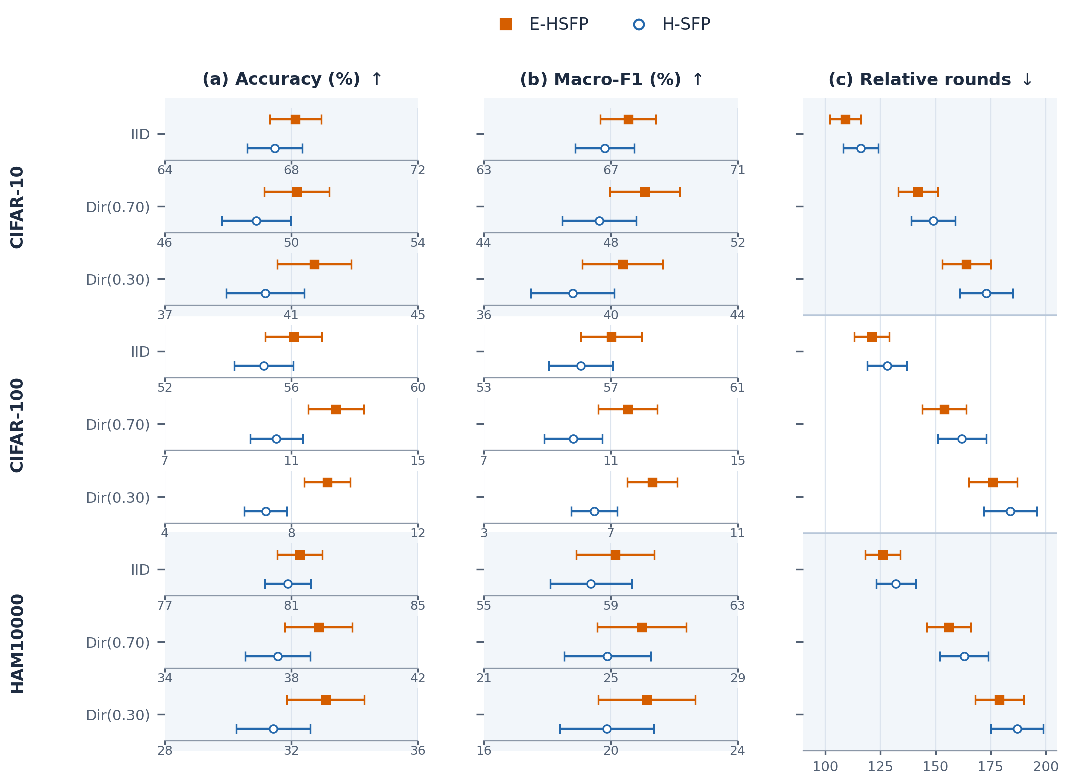
\includegraphics[width=\linewidth]{figures/fig_partition_comparison.pdf}
    \caption{Partition sensitivity reported as mean $\pm$ standard deviation for H-SFP and E-HSFP across 3 datasets. \reviewpurple{The plotting source describes these values as five-seed aggregates, but resolved per-seed 200-round records were not recovered locally.} Relative rounds use the run-specific validation criterion in Section~\ref{sec:experiments}.}
    \label{fig:partition_accuracy}
\end{figure}
Figure~\ref{fig:partition_accuracy} compares classification performance and training progress across nine dataset--partition settings. For \ehsfp{}, mean accuracy falls from 68.13\%, 56.07\%, and 81.27\% under IID to 41.73\%, 9.13\%, and 33.08\% under $\mathrm{Dir}(0.30)$ on CIFAR-10, CIFAR-100, and HAM10000, respectively. On HAM10000 IID, mean macro-F1 is 59.14\%, compared with mean accuracy of 81.27\%. Macro-F1 gives each class equal weight and complements accuracy on imbalanced data.

For CIFAR-100, the mean \ehsfp{} relative-round count rises from 121 under IID to 176 under $\mathrm{Dir}(0.30)$. Each count measures progress toward a run-specific threshold. Estimating the prototype drift defined in Section~\ref{sec:formulation} requires a separate comparison with fresh-prototype distributions. \reviewblue{The accuracy drop from IID to $\mathrm{Dir}(0.30)$ (e.g., from 56.07\% to 9.13\% on CIFAR-100) is far larger than any drop caused by masking or delay in Table~\ref{tab:robustness}. This pattern is consistent with Remark~\ref{rem:scatter_pooling} and Proposition~\ref{prop:weighting_shift}, under which label skew affects both the pooled covariance and the aggregated means, but this attribution has not been tested. The published H-SFP value at $T_{\mathrm{temp}}=0.5$ is $10.48\pm0.85\%$ for CIFAR-100 $\mathrm{Dir}(0.70)$~\cite{tran2026h}.} \reviewpurple{For \ehsfp{} at $T_{\mathrm{temp}}=0.5$, the table's former $13.02\pm0.80\%$ candidate conflicts with Figure~\ref{fig:partition_accuracy}'s $12.41\pm0.87\%$ candidate; neither is retained as a verified result.} \reviewred{[Evidence gap: excluding the unavailable $T_{\mathrm{temp}}=0.5$ cell, the populated \ehsfp{} CIFAR-100 $\mathrm{Dir}(0.70)$ temperature-sweep entries span $8.09$--$10.43\%$ and have no retained resolved per-seed 200-round records. The only locally retained CIFAR-100 \ehsfp{} $\mathrm{Dir}(0.30)$ and $\mathrm{Dir}(0.70)$ attempts are incomplete seed-0, 60-round runs at $T_{\mathrm{temp}}=0.1$. A matched common-temperature five-seed comparison is required before interpreting the partition gap.]}

\subsection{Configuration Contrasts}

Table~\ref{tab:ablation} compares replay, aggregation, and synthesis configurations. The reported full-synthesis row has mean accuracies 0.64, 0.42, and 0.40 percentage points above the diagonal PRC row in the reference, source-masking, and staleness conditions, respectively. The archive omits the exact generator and run-specific overrides for the full-synthesis row, so these differences describe the reported configurations.

Among the aggregation rows labeled $\memcap=0$, learned weighting has the highest mean accuracy in all three conditions. Its mean accuracy exceeds that of legacy uniform aggregation by 0.51, 0.64, and 0.43 percentage points in the reference, source-masking, and staleness conditions, respectively. The legacy rule also uses a different variance calculation (Section~\ref{sec:reliability}). In the same order, the reported full-synthesis row exceeds the learned-weighting row labeled $\memcap=0$ by 0.39, 1.35, and 1.61 percentage points.

Compared with the reported full-synthesis row, the row labeled $\memcap=20$ has 0.05 percentage points lower mean reference accuracy and 0.14 and 0.22 percentage points higher mean accuracy under source masking and staleness, respectively. Its mean relative-round count is two rounds higher. These differences describe archived configurations whose memory-control settings remain unresolved.

\subsection{Architecture, Client-Count, and Temperature Sensitivity}
\label{sec:evaluation_200}

Table~\ref{tab:sweep_200} reports accuracy across architectures, client counts, and temperatures. With VGG16 and IID partitions, \ehsfp{} attains mean accuracies of 79.03\% on HAM10000 and 26.89\% on ImageNet-1K. Across the CIFAR-100 IID client-count settings, mean accuracy falls from 68.49\% with 20 clients to 49.07\% with 500. On ImageNet-1K, it falls from 65.63\% with 20 clients to 29.37\% in the 200-client reference condition in Table~\ref{tab:main_classification}. \reviewpurple{Among the currently populated reported \ehsfp{} temperature cells in Table~\ref{tab:sweep_200}(d), $T_{\mathrm{temp}}=0.50$ has the highest mean in the three IID settings. $T_{\mathrm{temp}}=1.00$ has the highest mean among the populated alternatives in the three $\mathrm{Dir}(0.7)$ settings, but their $T_{\mathrm{temp}}=0.50$ cells are unavailable, so the table does not establish a single best temperature across all six settings.} \reviewblue{The table includes the published H-SFP $T_{\mathrm{temp}}=0.5$ column~\cite{tran2026h}.} \reviewpurple{The former \ehsfp{} $T_{\mathrm{temp}}=0.5$ candidates for CIFAR-10, CIFAR-100, and HAM10000 $\mathrm{Dir}(0.7)$ were $40.12\pm1.15\%$, $13.02\pm0.80\%$, and $38.12\pm1.03\%$ in the table, versus $50.17\pm1.03\%$, $12.41\pm0.87\%$, and $38.86\pm1.07\%$ in Figure~\ref{fig:partition_accuracy}. The available evidence cannot distinguish different configurations from transcription errors, so these discrepancies are classified as missing provenance.} \reviewred{[Evidence gap: no retained per-seed 200-round records independently verify the \ehsfp{} temperature cells. The three conflicting $T_{\mathrm{temp}}=0.5$, $\mathrm{Dir}(0.7)$ cells are therefore unavailable pending matched five-seed runs; the remaining reported aggregates also require original records or reruns before supporting a cross-temperature optimum.]}
